
%(BEGIN_QUESTION)
% Copyright 2010, Tony R. Kuphaldt, released under the Creative Commons Attribution License (v 1.0)
% This means you may do almost anything with this work of mine, so long as you give me proper credit

\noindent
{\bf Programming Challenge and Comparison -- Mixer motor auto-stop} 

\vskip 10pt

A batch mixing process in a manufacturing facility uses a mixer motor and a large ``paddlewheel'' to mix liquid ingredients to make a final product.  A PLC needs to run this motor for exactly 1500 turns of the paddlewheel and then automatically stop.  The motor needs to be able to start back up if the ``Start'' button is pressed again for the next batch:

$$\includegraphics[width=15.5cm]{i03688x01.eps}$$

\begin{itemize}
\item{} {\bf Inputs} 
\item{} Start pushbutton (momentary NO) -- {\it pushing this button closes the switch to energize the PLC input}
\item{} Stop pushbutton (momentary NC) -- {\it pushing this button opens the switch to de-energize the PLC input}
\item{} Proximity switch (NO) -- {\it one pulse per paddle revolution}
\end{itemize}

\begin{itemize}
\item{} {\bf Outputs} 
\item{} Motor contactor -- {\it energizing this PLC output starts the mixing motor}
\end{itemize}

Write a PLC program performing this function, and demonstrate its operation using switches connected to its inputs to simulate the discrete inputs in a real application.  

\vskip 10pt

When your program is complete and tested, capture a screen-shot of it as it appears on your computer, and prepare to present your program solution to the class in a review session for everyone to see and critique.  The purpose of this review session is to see multiple solutions to one problem, explore different programming techniques, and gain experience interpreting PLC programs others have written.  When presenting your program, prepare to discuss the following points:

\begin{itemize}
\item{} Identify the ``tag names'' or ``nicknames'' used within your program to label I/O and other bits in memory
\item{} Follow the sequence of operation in your program, simulating the system in action
\item{} Identify any special or otherwise non-standard instructions used in your program, and explain why you decided to take that approach
\item{} Show the comments placed in your program, to help explain how and why it works
\item{} How you designed the program (i.e. what steps you took to go from a concept to a working program)
\end{itemize}

\vskip 20pt \vbox{\hrule \hbox{\strut \vrule{} {\bf Suggestions for Socratic discussion} \vrule} \hrule}

\begin{itemize}
\item{} How can you test your program's basic operation without having to flick a switch {\it 1500 times} to simulate the full number of paddle revolutions?
\item{} Try writing your program so that the number of paddle-turns (1500) is not ``hard-coded'' into the PLC program, but rather resides in some memory location that may be altered without reprogramming the PLC.
\end{itemize}

\vfil

\underbar{file i03688}
\eject
%(END_QUESTION)





%(BEGIN_ANSWER)


%(END_ANSWER)





%(BEGIN_NOTES)

Sample program:

$$\includegraphics[width=15.5cm]{i03688x02.eps}$$










\vfil \eject

\noindent
{\bf Summary Quiz:}

(The recommended summary quiz is to have \underbar{each student} demonstrate their PLCs running this particular program)

%INDEX% PLC, programming challenge: mixer motor auto-stop (after so many turns)
%INDEX% Process: batch liquid mixing system (generic)

%(END_NOTES)


